\documentclass[9pt]{beamer}
\usetheme{cmepda}

\usepackage[utf8]{inputenc}
\usepackage[T1]{fontenc}

\graphicspath{{figures/}} 


\title{OOP introduction (2/2)}
\subtitle{Computing Methods for Experimental Physics and Data Analysis}
\date{Compiled on \today}
\author{A. Manfreda}
\institute[INFN]{INFN--Pisa}
\email{alberto.manfreda@pi.infn.it}


\begin{document}


\titleframe


\begin{frame}
  \frametitle{Introducing the Vector2d class}
  
  \begin{itemize}
    \item Suppose we want to create a class for managing 2D vectors
    \bigskip
    \item That's just for learning: there are already plenty of libraries for
          doing array operations - like numpy!
    \bigskip
    \item Anyway let's start coding some useful methods for it
  \end{itemize}
  
\end{frame}


\begin{frame}
  \frametitle{Introducing the Vector2d class}
  \framesubtitle{Naive version}
  \begin{Verbatim}[label=\makebox{\url{https://github.com/lucabaldini/cmepda/tree/master/slides/latex/snippets/vector2d\_naive.py}},commandchars=\\\{\}]
\PY{k+kn}{import} \PY{n+nn}{math}

\PY{k}{class} \PY{n+nc}{Vector2d}\PY{p}{:}
    \PY{l+s+sd}{\PYZdq{}\PYZdq{}\PYZdq{} Class representing a Vector2d. We use float() to make sure of storing}
\PY{l+s+sd}{    the coordinates in the correct format \PYZdq{}\PYZdq{}\PYZdq{}}   
    \PY{k}{def} \PY{n+nf+fm}{\PYZus{}\PYZus{}init\PYZus{}\PYZus{}}\PY{p}{(}\PY{n+nb+bp}{self}\PY{p}{,} \PY{n}{x}\PY{p}{,} \PY{n}{y}\PY{p}{)}\PY{p}{:}
        \PY{n+nb+bp}{self}\PY{o}{.}\PY{n}{x} \PY{o}{=} \PY{n+nb}{float}\PY{p}{(}\PY{n}{x}\PY{p}{)}
        \PY{n+nb+bp}{self}\PY{o}{.}\PY{n}{y} \PY{o}{=} \PY{n+nb}{float}\PY{p}{(}\PY{n}{y}\PY{p}{)}
   
    \PY{k}{def} \PY{n+nf}{module}\PY{p}{(}\PY{n+nb+bp}{self}\PY{p}{)}\PY{p}{:}
        \PY{k}{return} \PY{n}{math}\PY{o}{.}\PY{n}{sqrt}\PY{p}{(}\PY{n+nb+bp}{self}\PY{o}{.}\PY{n}{x}\PY{o}{*}\PY{o}{*}\PY{l+m+mi}{2} \PY{o}{+} \PY{n+nb+bp}{self}\PY{o}{.}\PY{n}{y}\PY{o}{*}\PY{o}{*}\PY{l+m+mi}{2}\PY{p}{)}
       
    \PY{k}{def} \PY{n+nf}{nice\PYZus{}print}\PY{p}{(}\PY{n+nb+bp}{self}\PY{p}{)}\PY{p}{:}
        \PY{k}{print} \PY{p}{(}\PY{l+s+s1}{\PYZsq{}}\PY{l+s+s1}{Vector2d(\PYZob{}\PYZcb{}, \PYZob{}\PYZcb{})}\PY{l+s+s1}{\PYZsq{}}\PY{o}{.}\PY{n}{format}\PY{p}{(}\PY{n+nb+bp}{self}\PY{o}{.}\PY{n}{x}\PY{p}{,} \PY{n+nb+bp}{self}\PY{o}{.}\PY{n}{y}\PY{p}{)}\PY{p}{)}
   
    \PY{k}{def} \PY{n+nf}{add}\PY{p}{(}\PY{n+nb+bp}{self}\PY{p}{,} \PY{n}{other}\PY{p}{)}\PY{p}{:}
        \PY{k}{return} \PY{n}{Vector2d}\PY{p}{(}\PY{n+nb+bp}{self}\PY{o}{.}\PY{n}{x} \PY{o}{+} \PY{n}{other}\PY{o}{.}\PY{n}{x}\PY{p}{,} \PY{n+nb+bp}{self}\PY{o}{.}\PY{n}{y} \PY{o}{+} \PY{n}{other}\PY{o}{.}\PY{n}{y}\PY{p}{)}
       
\PY{n}{v} \PY{o}{=} \PY{n}{Vector2d}\PY{p}{(}\PY{l+m+mf}{3.}\PY{p}{,} \PY{o}{\PYZhy{}}\PY{l+m+mf}{1.}\PY{p}{)}
\PY{n}{v}\PY{o}{.}\PY{n}{nice\PYZus{}print}\PY{p}{(}\PY{p}{)}
\PY{k}{print}\PY{p}{(}\PY{n}{v}\PY{o}{.}\PY{n}{module}\PY{p}{(}\PY{p}{)}\PY{p}{)}
\PY{n}{z} \PY{o}{=} \PY{n}{Vector2d}\PY{p}{(}\PY{l+m+mf}{1.}\PY{p}{,} \PY{l+m+mf}{1.5}\PY{p}{)}
\PY{n}{t} \PY{o}{=} \PY{n}{v}\PY{o}{.}\PY{n}{add}\PY{p}{(}\PY{n}{z}\PY{p}{)}
\PY{n}{t}\PY{o}{.}\PY{n}{nice\PYZus{}print}\PY{p}{(}\PY{p}{)}

[Output]
Vector2d(3.0, -1.0)
3.1622776601683795
Vector2d(4.0, 0.5)
\end{Verbatim}
\end{frame}


\begin{frame}
  \frametitle{The vector problem}
  
  \begin{itemize}
    \item This kind of works but\dots... isn't that ugly?
    \medskip
    \item Look at the lines \emph{v.nice\_print()} or \emph{v.module().}
          It would be far more readible to just do \emph{print(v)} and \emph{abs(v)}
    \medskip
    \item And what about \emph{t = v.add(z)}? Why not \emph{t = v + z}?
    \medskip
    \item In Python there is a tool that allows you to do just that: \alert{special methods}
    \medskip
    \item Last lesson we saw that special methods (or dunder methods or 
          magic methods) are methods like \emph{\_\_init\_\_} and got a special
          treatment by the Python interpeter
    \medskip
    \item There are a few tens of special methods in Python. Let's see how they work
  \end{itemize}
  
\end{frame}

  
\begin{frame}
  \frametitle{Vector2d}
  \framesubtitle{A first look at special methods}
  \begin{Verbatim}[label=\makebox{\url{https://bitbucket.org/lbaldini/programming/src/tip/snippets/vector2d\_2.py}},commandchars=\\\{\}]
\PY{k+kn}{import} \PY{n+nn}{math}

\PY{k}{class} \PY{n+nc}{Vector2d}\PY{p}{:}
    \PY{l+s+sd}{\PYZdq{}\PYZdq{}\PYZdq{} Class representing a Vector2d \PYZdq{}\PYZdq{}\PYZdq{}}   
    \PY{k}{def} \PY{n+nf+fm}{\PYZus{}\PYZus{}init\PYZus{}\PYZus{}}\PY{p}{(}\PY{n+nb+bp}{self}\PY{p}{,} \PY{n}{x}\PY{p}{,} \PY{n}{y}\PY{p}{)}\PY{p}{:}
        \PY{n+nb+bp}{self}\PY{o}{.}\PY{n}{x} \PY{o}{=} \PY{n}{x}
        \PY{n+nb+bp}{self}\PY{o}{.}\PY{n}{y} \PY{o}{=} \PY{n}{y}
   
    \PY{k}{def} \PY{n+nf+fm}{\PYZus{}\PYZus{}abs\PYZus{}\PYZus{}}\PY{p}{(}\PY{n+nb+bp}{self}\PY{p}{)}\PY{p}{:}
        \PY{c+c1}{\PYZsh{} Special method!}
        \PY{k}{return} \PY{n}{math}\PY{o}{.}\PY{n}{sqrt}\PY{p}{(}\PY{n+nb+bp}{self}\PY{o}{.}\PY{n}{x}\PY{o}{*}\PY{o}{*}\PY{l+m+mi}{2} \PY{o}{+} \PY{n+nb+bp}{self}\PY{o}{.}\PY{n}{y}\PY{o}{*}\PY{o}{*}\PY{l+m+mi}{2}\PY{p}{)}
     
\PY{n}{v} \PY{o}{=} \PY{n}{Vector2d}\PY{p}{(}\PY{l+m+mf}{3.}\PY{p}{,} \PY{o}{\PYZhy{}}\PY{l+m+mf}{1.}\PY{p}{)}
\PY{c+c1}{\PYZsh{} The Python interpeter automatically replace abs(v) with Vector2d.\PYZus{}\PYZus{}abs\PYZus{}\PYZus{}(v)}
\PY{k}{print}\PY{p}{(}\PY{n+nb}{abs}\PY{p}{(}\PY{n}{v}\PY{p}{)}\PY{p}{)}

[Output]
3.1622776601683795
\end{Verbatim}
\end{frame}


\begin{frame}
  \frametitle{More on special methods}
  
  \begin{itemize}
    \item And what about \emph{print()}?
    \item There are actually two special methods used for that: \emph{\_\_str\_\_} and \emph{\_\_repr\_\_}
    \medskip
    \item \emph{\_\_str\_\_} is meant to return a concise string for the user; it is called with \emph{str()}
    \medskip
    \item \emph{\_\_repr\_\_} is meant to return a richer output for debug. It is called with \emph{repr()}
    \medskip
    \item \emph{print()} automatically tries to get a string out of the object using \emph{\_\_str\_\_}
    \medskip
    \item If there isn't one, it searches for \emph{\_\_repr\_\_}. A defealut \emph{\_\_repr\_\_}
          is automatically generated for you, if you haven't defined one
  \end{itemize}
  
\end{frame}


\begin{frame}
  \frametitle{Vector2d}
  \framesubtitle{\emph{\_\_str\_\_} and \emph{\_\_repr\_\_}}
  \begin{Verbatim}[label=\makebox{\url{https://bitbucket.org/lbaldini/programming/src/tip/snippets/vector2d\_printable.py}},commandchars=\\\{\}]
\PY{k}{class} \PY{n+nc}{Vector2d}\PY{p}{:}
    \PY{l+s+sd}{\PYZdq{}\PYZdq{}\PYZdq{} Class representing a Vector2d \PYZdq{}\PYZdq{}\PYZdq{}}   
    \PY{k}{def} \PY{n+nf+fm}{\PYZus{}\PYZus{}init\PYZus{}\PYZus{}}\PY{p}{(}\PY{n+nb+bp}{self}\PY{p}{,} \PY{n}{x}\PY{p}{,} \PY{n}{y}\PY{p}{)}\PY{p}{:}
        \PY{n+nb+bp}{self}\PY{o}{.}\PY{n}{x} \PY{o}{=} \PY{n+nb}{float}\PY{p}{(}\PY{n}{x}\PY{p}{)}
        \PY{n+nb+bp}{self}\PY{o}{.}\PY{n}{y} \PY{o}{=} \PY{n+nb}{float}\PY{p}{(}\PY{n}{y}\PY{p}{)}
   
    \PY{k}{def} \PY{n+nf+fm}{\PYZus{}\PYZus{}repr\PYZus{}\PYZus{}}\PY{p}{(}\PY{n+nb+bp}{self}\PY{p}{)}\PY{p}{:}
        \PY{c+c1}{\PYZsh{} We don\PYZsq{}t want to hard\PYZhy{}code the class name, so we dynamically get it}
        \PY{n}{class\PYZus{}name} \PY{o}{=} \PY{n+nb}{type}\PY{p}{(}\PY{n+nb+bp}{self}\PY{p}{)}\PY{o}{.}\PY{n+nv+vm}{\PYZus{}\PYZus{}name\PYZus{}\PYZus{}}
        \PY{k}{return} \PY{p}{(}\PY{l+s+s1}{\PYZsq{}}\PY{l+s+s1}{\PYZob{}\PYZcb{}(\PYZob{}\PYZcb{}, \PYZob{}\PYZcb{})}\PY{l+s+s1}{\PYZsq{}}\PY{o}{.}\PY{n}{format}\PY{p}{(}\PY{n}{class\PYZus{}name}\PY{p}{,} \PY{n+nb+bp}{self}\PY{o}{.}\PY{n}{x}\PY{p}{,} \PY{n+nb+bp}{self}\PY{o}{.}\PY{n}{y}\PY{p}{)}\PY{p}{)}
        
    \PY{k}{def} \PY{n+nf+fm}{\PYZus{}\PYZus{}str\PYZus{}\PYZus{}}\PY{p}{(}\PY{n+nb+bp}{self}\PY{p}{)}\PY{p}{:}
        \PY{l+s+sd}{\PYZdq{}\PYZdq{}\PYZdq{} We convert the coordinates to a tuple so that we can reuse the}
\PY{l+s+sd}{        \PYZus{}\PYZus{}str\PYZus{}\PYZus{} method of tuples, which already provides a nice formatting.}
\PY{l+s+sd}{        Notice the two parenthesis: this line is equivalent to:}
\PY{l+s+sd}{        temp\PYZus{}tuple = (self.x, self.y)}
\PY{l+s+sd}{        return str(temp\PYZus{}tuple)}
\PY{l+s+sd}{        \PYZdq{}\PYZdq{}\PYZdq{}}
        \PY{k}{return} \PY{n+nb}{str}\PY{p}{(}\PY{p}{(}\PY{n+nb+bp}{self}\PY{o}{.}\PY{n}{x}\PY{p}{,} \PY{n+nb+bp}{self}\PY{o}{.}\PY{n}{y}\PY{p}{)}\PY{p}{)}
     
\PY{n}{v} \PY{o}{=} \PY{n}{Vector2d}\PY{p}{(}\PY{l+m+mf}{3.}\PY{p}{,} \PY{o}{\PYZhy{}}\PY{l+m+mf}{1.}\PY{p}{)}
\PY{k}{print}\PY{p}{(}\PY{n}{v}\PY{p}{)} \PY{c+c1}{\PYZsh{} Is the same as print(str(v))}
\PY{k}{print}\PY{p}{(}\PY{n+nb}{repr}\PY{p}{(}\PY{n}{v}\PY{p}{)}\PY{p}{)}
\PY{k}{print}\PY{p}{(}\PY{l+s+s1}{\PYZsq{}}\PY{l+s+s1}{I got \PYZob{}\PYZcb{} with \PYZus{}\PYZus{}str\PYZus{}\PYZus{} and \PYZob{}!r\PYZcb{} with \PYZus{}\PYZus{}repr\PYZus{}\PYZus{}}\PY{l+s+s1}{\PYZsq{}}\PY{o}{.}\PY{n}{format}\PY{p}{(}\PY{n}{v}\PY{p}{,} \PY{n}{v}\PY{p}{)}\PY{p}{)}

[Output]
(3.0, -1.0)
Vector2d(3.0, -1.0)
I got (3.0, -1.0) with __str__ and Vector2d(3.0, -1.0) with __repr__
\end{Verbatim}
\end{frame}


\begin{frame}
  \frametitle{Vector2d}
  \framesubtitle{Mathematical operations}
  \begin{Verbatim}[label=\makebox{\url{https://bitbucket.org/lbaldini/programming/src/tip/snippets/vector2d\_math.py}},commandchars=\\\{\}]
\PY{k}{class} \PY{n+nc}{Vector2d}\PY{p}{:}
    \PY{l+s+sd}{\PYZdq{}\PYZdq{}\PYZdq{} Class representing a Vector2d \PYZdq{}\PYZdq{}\PYZdq{}}   
    \PY{k}{def} \PY{n+nf+fm}{\PYZus{}\PYZus{}init\PYZus{}\PYZus{}}\PY{p}{(}\PY{n+nb+bp}{self}\PY{p}{,} \PY{n}{x}\PY{p}{,} \PY{n}{y}\PY{p}{)}\PY{p}{:}
        \PY{n+nb+bp}{self}\PY{o}{.}\PY{n}{x} \PY{o}{=} \PY{n+nb}{float}\PY{p}{(}\PY{n}{x}\PY{p}{)}
        \PY{n+nb+bp}{self}\PY{o}{.}\PY{n}{y} \PY{o}{=} \PY{n+nb}{float}\PY{p}{(}\PY{n}{y}\PY{p}{)}
   
    \PY{k}{def} \PY{n+nf+fm}{\PYZus{}\PYZus{}add\PYZus{}\PYZus{}}\PY{p}{(}\PY{n+nb+bp}{self}\PY{p}{,} \PY{n}{other}\PY{p}{)}\PY{p}{:}
        \PY{k}{return} \PY{n}{Vector2d}\PY{p}{(}\PY{n+nb+bp}{self}\PY{o}{.}\PY{n}{x} \PY{o}{+} \PY{n}{other}\PY{o}{.}\PY{n}{x}\PY{p}{,} \PY{n+nb+bp}{self}\PY{o}{.}\PY{n}{y} \PY{o}{+} \PY{n}{other}\PY{o}{.}\PY{n}{y}\PY{p}{)}
    
    \PY{k}{def} \PY{n+nf+fm}{\PYZus{}\PYZus{}mul\PYZus{}\PYZus{}}\PY{p}{(}\PY{n+nb+bp}{self}\PY{p}{,} \PY{n}{scalar}\PY{p}{)}\PY{p}{:}
        \PY{k}{return} \PY{n}{Vector2d}\PY{p}{(}\PY{n}{scalar} \PY{o}{*} \PY{n+nb+bp}{self}\PY{o}{.}\PY{n}{x}\PY{p}{,} \PY{n}{scalar} \PY{o}{*} \PY{n+nb+bp}{self}\PY{o}{.}\PY{n}{y}\PY{p}{)}
        
    \PY{k}{def} \PY{n+nf+fm}{\PYZus{}\PYZus{}rmul\PYZus{}\PYZus{}}\PY{p}{(}\PY{n+nb+bp}{self}\PY{p}{,} \PY{n}{scalar}\PY{p}{)}\PY{p}{:}
        \PY{c+c1}{\PYZsh{} Right multiplication \PYZhy{} because a * Vector is different from Vector * a}
        \PY{k}{return} \PY{n+nb+bp}{self} \PY{o}{*} \PY{n}{scalar} \PY{c+c1}{\PYZsh{} We just call \PYZus{}\PYZus{}mul\PYZus{}\PYZus{}, no code duplication!}
        
    \PY{k}{def} \PY{n+nf+fm}{\PYZus{}\PYZus{}str\PYZus{}\PYZus{}}\PY{p}{(}\PY{n+nb+bp}{self}\PY{p}{)}\PY{p}{:}
        \PY{c+c1}{\PYZsh{} We keep this to show the results nicely}
        \PY{k}{return} \PY{n+nb}{str}\PY{p}{(}\PY{p}{(}\PY{n+nb+bp}{self}\PY{o}{.}\PY{n}{x}\PY{p}{,} \PY{n+nb+bp}{self}\PY{o}{.}\PY{n}{y}\PY{p}{)}\PY{p}{)}
     
\PY{n}{v}\PY{p}{,} \PY{n}{z} \PY{o}{=} \PY{n}{Vector2d}\PY{p}{(}\PY{l+m+mf}{3.}\PY{p}{,} \PY{o}{\PYZhy{}}\PY{l+m+mf}{1.}\PY{p}{)}\PY{p}{,} \PY{n}{Vector2d}\PY{p}{(}\PY{o}{\PYZhy{}}\PY{l+m+mf}{5.}\PY{p}{,} \PY{l+m+mf}{1.}\PY{p}{)}
\PY{k}{print}\PY{p}{(}\PY{n}{v}\PY{o}{+}\PY{n}{z}\PY{p}{)}
\PY{k}{print}\PY{p}{(}\PY{l+m+mi}{3} \PY{o}{*} \PY{n}{v}\PY{p}{)}
\PY{k}{print}\PY{p}{(}\PY{n}{z} \PY{o}{*} \PY{l+m+mi}{5}\PY{p}{)}

[Output]
(-2.0, 0.0)
(9.0, -3.0)
(-25.0, 5.0)
\end{Verbatim}
\end{frame}


\begin{frame}
  \frametitle{Vector2d}
  \framesubtitle{In-place operations}
  \begin{Verbatim}[label=\makebox{\url{https://github.com/lucabaldini/cmepda/tree/master/slides/latex/snippets/vector2d\_inplace.py}},commandchars=\\\{\}]
\PY{k}{class} \PY{n+nc}{Vector2d}\PY{p}{:}
    \PY{l+s+sd}{\PYZdq{}\PYZdq{}\PYZdq{} Class representing a Vector2d \PYZdq{}\PYZdq{}\PYZdq{}}   
    \PY{k}{def} \PY{n+nf+fm}{\PYZus{}\PYZus{}init\PYZus{}\PYZus{}}\PY{p}{(}\PY{n+nb+bp}{self}\PY{p}{,} \PY{n}{x}\PY{p}{,} \PY{n}{y}\PY{p}{)}\PY{p}{:}
        \PY{n+nb+bp}{self}\PY{o}{.}\PY{n}{x} \PY{o}{=} \PY{n+nb}{float}\PY{p}{(}\PY{n}{x}\PY{p}{)}
        \PY{n+nb+bp}{self}\PY{o}{.}\PY{n}{y} \PY{o}{=} \PY{n+nb}{float}\PY{p}{(}\PY{n}{y}\PY{p}{)}
    
    \PY{k}{def} \PY{n+nf+fm}{\PYZus{}\PYZus{}iadd\PYZus{}\PYZus{}}\PY{p}{(}\PY{n+nb+bp}{self}\PY{p}{,} \PY{n}{other}\PY{p}{)}\PY{p}{:}
        \PY{n+nb+bp}{self}\PY{o}{.}\PY{n}{x} \PY{o}{+}\PY{o}{=} \PY{n}{other}\PY{o}{.}\PY{n}{x}
        \PY{n+nb+bp}{self}\PY{o}{.}\PY{n}{y} \PY{o}{+}\PY{o}{=} \PY{n}{other}\PY{o}{.}\PY{n}{y}
        \PY{k}{return} \PY{n+nb+bp}{self}
        
    \PY{k}{def} \PY{n+nf+fm}{\PYZus{}\PYZus{}imul\PYZus{}\PYZus{}}\PY{p}{(}\PY{n+nb+bp}{self}\PY{p}{,} \PY{n}{other}\PY{p}{)}\PY{p}{:}
        \PY{n+nb+bp}{self}\PY{o}{.}\PY{n}{x} \PY{o}{*}\PY{o}{=} \PY{n}{other}\PY{o}{.}\PY{n}{x}
        \PY{n+nb+bp}{self}\PY{o}{.}\PY{n}{y} \PY{o}{*}\PY{o}{=} \PY{n}{other}\PY{o}{.}\PY{n}{y}
        \PY{k}{return} \PY{n+nb+bp}{self}
        
    \PY{k}{def} \PY{n+nf+fm}{\PYZus{}\PYZus{}str\PYZus{}\PYZus{}}\PY{p}{(}\PY{n+nb+bp}{self}\PY{p}{)}\PY{p}{:}
        \PY{k}{return} \PY{n+nb}{str}\PY{p}{(}\PY{p}{(}\PY{n+nb+bp}{self}\PY{o}{.}\PY{n}{x}\PY{p}{,} \PY{n+nb+bp}{self}\PY{o}{.}\PY{n}{y}\PY{p}{)}\PY{p}{)}
     
\PY{n}{v} \PY{o}{=} \PY{n}{Vector2d}\PY{p}{(}\PY{l+m+mf}{3.}\PY{p}{,} \PY{o}{\PYZhy{}}\PY{l+m+mf}{1.}\PY{p}{)}
\PY{n}{z} \PY{o}{=} \PY{n}{Vector2d}\PY{p}{(}\PY{o}{\PYZhy{}}\PY{l+m+mf}{5.}\PY{p}{,} \PY{l+m+mf}{1.}\PY{p}{)}
\PY{n}{v} \PY{o}{+}\PY{o}{=} \PY{n}{z}
\PY{k}{print}\PY{p}{(}\PY{n}{v}\PY{p}{)}
\PY{n}{v} \PY{o}{*}\PY{o}{=} \PY{n}{z}
\PY{k}{print}\PY{p}{(}\PY{n}{v}\PY{p}{)}

[Output]
(-2.0, 0.0)
(10.0, 0.0)
\end{Verbatim}
\end{frame}


\begin{frame}
  \frametitle{Vector2d}
  \framesubtitle{Comparisons}
  \begin{Verbatim}[label=\makebox{\url{https://github.com/lucabaldini/cmepda/tree/master/slides/latex/snippets/vector2d\_comparable.py}},commandchars=\\\{\}]
\PY{k+kn}{import} \PY{n+nn}{math}

\PY{k}{class} \PY{n+nc}{Vector2d}\PY{p}{:}
    \PY{l+s+sd}{\PYZdq{}\PYZdq{}\PYZdq{} Class representing a Vector2d \PYZdq{}\PYZdq{}\PYZdq{}}   
    \PY{k}{def} \PY{n+nf+fm}{\PYZus{}\PYZus{}init\PYZus{}\PYZus{}}\PY{p}{(}\PY{n+nb+bp}{self}\PY{p}{,} \PY{n}{x}\PY{p}{,} \PY{n}{y}\PY{p}{)}\PY{p}{:}
        \PY{n+nb+bp}{self}\PY{o}{.}\PY{n}{x} \PY{o}{=} \PY{n+nb}{float}\PY{p}{(}\PY{n}{x}\PY{p}{)}
        \PY{n+nb+bp}{self}\PY{o}{.}\PY{n}{y} \PY{o}{=} \PY{n+nb}{float}\PY{p}{(}\PY{n}{y}\PY{p}{)}
    
    \PY{k}{def} \PY{n+nf+fm}{\PYZus{}\PYZus{}abs\PYZus{}\PYZus{}}\PY{p}{(}\PY{n+nb+bp}{self}\PY{p}{)}\PY{p}{:}
        \PY{c+c1}{\PYZsh{} We need this for \PYZus{}\PYZus{}eq\PYZus{}\PYZus{}}
        \PY{k}{return} \PY{n}{math}\PY{o}{.}\PY{n}{sqrt}\PY{p}{(}\PY{n+nb+bp}{self}\PY{o}{.}\PY{n}{x}\PY{o}{*}\PY{o}{*}\PY{l+m+mi}{2} \PY{o}{+} \PY{n+nb+bp}{self}\PY{o}{.}\PY{n}{y}\PY{o}{*}\PY{o}{*}\PY{l+m+mi}{2}\PY{p}{)}
    
    \PY{k}{def} \PY{n+nf+fm}{\PYZus{}\PYZus{}eq\PYZus{}\PYZus{}}\PY{p}{(}\PY{n+nb+bp}{self}\PY{p}{,} \PY{n}{other}\PY{p}{)}\PY{p}{:}
        \PY{c+c1}{\PYZsh{} Implement the \PYZsq{}==\PYZsq{} operator}
        \PY{k}{return} \PY{p}{(}\PY{p}{(}\PY{n+nb+bp}{self}\PY{o}{.}\PY{n}{x}\PY{p}{,} \PY{n+nb+bp}{self}\PY{o}{.}\PY{n}{y}\PY{p}{)} \PY{o}{==} \PY{p}{(}\PY{n}{other}\PY{o}{.}\PY{n}{x}\PY{p}{,} \PY{n}{other}\PY{o}{.}\PY{n}{y}\PY{p}{)}\PY{p}{)}
        
    \PY{k}{def} \PY{n+nf+fm}{\PYZus{}\PYZus{}ge\PYZus{}\PYZus{}}\PY{p}{(}\PY{n+nb+bp}{self}\PY{p}{,} \PY{n}{other}\PY{p}{)}\PY{p}{:}
        \PY{c+c1}{\PYZsh{} Implement the \PYZsq{}\PYZgt{}=\PYZsq{} operator}
        \PY{k}{return} \PY{n+nb}{abs}\PY{p}{(}\PY{n+nb+bp}{self}\PY{p}{)} \PY{o}{\PYZgt{}}\PY{o}{=} \PY{n+nb}{abs}\PY{p}{(}\PY{n}{other}\PY{p}{)}
        
    \PY{k}{def} \PY{n+nf+fm}{\PYZus{}\PYZus{}lt\PYZus{}\PYZus{}}\PY{p}{(}\PY{n+nb+bp}{self}\PY{p}{,} \PY{n}{other}\PY{p}{)}\PY{p}{:}
        \PY{c+c1}{\PYZsh{} Implement the \PYZsq{}\PYZlt{}\PYZsq{} operator }
        \PY{k}{return} \PY{n+nb}{abs}\PY{p}{(}\PY{n+nb+bp}{self}\PY{p}{)} \PY{o}{\PYZlt{}} \PY{n+nb}{abs}\PY{p}{(}\PY{n}{other}\PY{p}{)}
        
    \PY{k}{def} \PY{n+nf+fm}{\PYZus{}\PYZus{}repr\PYZus{}\PYZus{}}\PY{p}{(}\PY{n+nb+bp}{self}\PY{p}{)}\PY{p}{:}
        \PY{c+c1}{\PYZsh{} We define \PYZus{}\PYZus{}repr\PYZus{}\PYZus{} for showing the results nicely}
        \PY{n}{class\PYZus{}name} \PY{o}{=} \PY{n+nb}{type}\PY{p}{(}\PY{n+nb+bp}{self}\PY{p}{)}\PY{o}{.}\PY{n+nv+vm}{\PYZus{}\PYZus{}name\PYZus{}\PYZus{}}
        \PY{k}{return} \PY{p}{(}\PY{l+s+s1}{\PYZsq{}}\PY{l+s+s1}{\PYZob{}\PYZcb{}(\PYZob{}\PYZcb{}, \PYZob{}\PYZcb{})}\PY{l+s+s1}{\PYZsq{}}\PY{o}{.}\PY{n}{format}\PY{p}{(}\PY{n}{class\PYZus{}name}\PY{p}{,} \PY{n+nb+bp}{self}\PY{o}{.}\PY{n}{x}\PY{p}{,} \PY{n+nb+bp}{self}\PY{o}{.}\PY{n}{y}\PY{p}{)}\PY{p}{)}
\end{Verbatim}
\end{frame}


\begin{frame}
  \frametitle{Vector2d}
  \framesubtitle{Comparisons}
  \begin{Verbatim}[label=\makebox{\url{https://bitbucket.org/lbaldini/programming/src/tip/snippets/test\_vector2d\_comparable.py}},commandchars=\\\{\}]
\PY{k+kn}{from} \PY{n+nn}{vector2d\PYZus{}comparable} \PY{k+kn}{import} \PY{n}{Vector2d}

\PY{n}{v}\PY{p}{,} \PY{n}{z} \PY{o}{=} \PY{n}{Vector2d}\PY{p}{(}\PY{l+m+mf}{3.}\PY{p}{,} \PY{o}{\PYZhy{}}\PY{l+m+mf}{1.}\PY{p}{)}\PY{p}{,} \PY{n}{Vector2d}\PY{p}{(}\PY{l+m+mf}{3.}\PY{p}{,} \PY{l+m+mf}{1.}\PY{p}{)}
\PY{k}{print}\PY{p}{(}\PY{n}{v} \PY{o}{\PYZgt{}}\PY{o}{=} \PY{n}{z}\PY{p}{,} \PY{n}{v} \PY{o}{==} \PY{n}{z}\PY{p}{,} \PY{n}{v} \PY{o}{\PYZlt{}} \PY{n}{z}\PY{p}{)}
\PY{c+c1}{\PYZsh{} This works even if we don\PYZsq{}t define the \PYZus{}\PYZus{}gt\PYZus{}\PYZus{} method explicitly}
\PY{k}{print}\PY{p}{(}\PY{n}{v} \PY{o}{\PYZgt{}} \PY{n}{z}\PY{p}{)}

\PY{n}{vector\PYZus{}list} \PY{o}{=} \PY{p}{[}\PY{n}{Vector2d}\PY{p}{(}\PY{l+m+mf}{3.}\PY{p}{,} \PY{o}{\PYZhy{}}\PY{l+m+mf}{1.}\PY{p}{)}\PY{p}{,} \PY{n}{Vector2d}\PY{p}{(}\PY{o}{\PYZhy{}}\PY{l+m+mf}{5.}\PY{p}{,} \PY{l+m+mf}{1.}\PY{p}{)}\PY{p}{,} \PY{n}{Vector2d}\PY{p}{(}\PY{l+m+mf}{3.}\PY{p}{,} \PY{l+m+mf}{0.}\PY{p}{)}\PY{p}{]}
\PY{k}{print}\PY{p}{(}\PY{n}{vector\PYZus{}list}\PY{p}{)}
\PY{c+c1}{\PYZsh{} Tho make the following line work we need to implement either \PYZus{}\PYZus{}ge\PYZus{}\PYZus{} and \PYZus{}\PYZus{}lt\PYZus{}\PYZus{}}
\PY{c+c1}{\PYZsh{} or \PYZus{}\PYZus{}gt\PYZus{}\PYZus{} and \PYZus{}\PYZus{}le\PYZus{}\PYZus{} (we need a complementary pair of operator)}
\PY{n}{vector\PYZus{}list}\PY{o}{.}\PY{n}{sort}\PY{p}{(}\PY{p}{)}
\PY{k}{print}\PY{p}{(}\PY{n}{vector\PYZus{}list}\PY{p}{)}
\PY{c+c1}{\PYZsh{} Note: we got the full power of timsort for free! Nice :)}

[Output]
True False False
False
[Vector2d(3.0, -1.0), Vector2d(-5.0, 1.0), Vector2d(3.0, 0.0)]
[Vector2d(3.0, 0.0), Vector2d(3.0, -1.0), Vector2d(-5.0, 1.0)]
\end{Verbatim}
\end{frame}


\begin{frame}
  \frametitle{An hashable Vector2d}
  
  \begin{itemize}
    \item Ok now let's try to make our vector2d \emph{hashable}
    \medskip
    \item Hashable objects can be put in \emph{sets} and used as keys for 
          dictionaries
    \medskip
    \item To make an object hashable we need to fullfill 3 requirements:
    \smallskip
    \begin{itemize}
      \item It has to be immutable - otherwise you may not retrieve the correct hash
      \smallskip
      \item It needs to implement a \emph{\_\_eq\_\_} function, so one can compare
            objects of this class
      \smallskip
      \item It needs a (reasonable) \emph{\_\_hash\_\_} function
    \end{itemize}
    \medskip
    \item Rules for a good hash function:
    \smallskip
    \begin{itemize}
      \item Must return the same value for objects that compare as equal
      \smallskip
      \item Should rarely return the same value for different objects
      \smallskip
      \item Should sample the result space uniformly
    \end{itemize}
    
  \end{itemize}
  
\end{frame}


\begin{frame}
  \frametitle{Vector2d}
  \framesubtitle{Hashable version}
  \begin{Verbatim}[label=\makebox{\url{https://bitbucket.org/lbaldini/programming/src/tip/snippets/vector2d\_hashable.py}},commandchars=\\\{\}]
\PY{k}{class} \PY{n+nc}{Vector2d}\PY{p}{:}
    \PY{l+s+sd}{\PYZdq{}\PYZdq{}\PYZdq{} Class representing a Vector2d \PYZdq{}\PYZdq{}\PYZdq{}}   
    \PY{k}{def} \PY{n+nf+fm}{\PYZus{}\PYZus{}init\PYZus{}\PYZus{}}\PY{p}{(}\PY{n+nb+bp}{self}\PY{p}{,} \PY{n}{x}\PY{p}{,} \PY{n}{y}\PY{p}{)}\PY{p}{:}
        \PY{l+s+sd}{\PYZdq{}\PYZdq{}\PYZdq{}\PYZdq{} We tell the user that x and y are private\PYZdq{}\PYZdq{}\PYZdq{}}
        \PY{n+nb+bp}{self}\PY{o}{.}\PY{n}{\PYZus{}x} \PY{o}{=} \PY{n+nb}{float}\PY{p}{(}\PY{n}{x}\PY{p}{)}
        \PY{n+nb+bp}{self}\PY{o}{.}\PY{n}{\PYZus{}y} \PY{o}{=} \PY{n+nb}{float}\PY{p}{(}\PY{n}{y}\PY{p}{)}
    
    \PY{n+nd}{@property}
    \PY{k}{def} \PY{n+nf}{x}\PY{p}{(}\PY{n+nb+bp}{self}\PY{p}{)}\PY{p}{:}
        \PY{l+s+sd}{\PYZdq{}\PYZdq{}\PYZdq{} Provides read only access to x \PYZhy{} since there is no setter\PYZdq{}\PYZdq{}\PYZdq{}}
        \PY{k}{return} \PY{n+nb+bp}{self}\PY{o}{.}\PY{n}{\PYZus{}x}
        
    \PY{n+nd}{@property}
    \PY{k}{def} \PY{n+nf}{y}\PY{p}{(}\PY{n+nb+bp}{self}\PY{p}{)}\PY{p}{:}
        \PY{l+s+sd}{\PYZdq{}\PYZdq{}\PYZdq{} Provides read only access to y \PYZhy{} since there is no setter\PYZdq{}\PYZdq{}\PYZdq{}}
        \PY{k}{return} \PY{n+nb+bp}{self}\PY{o}{.}\PY{n}{\PYZus{}y}
    
    \PY{k}{def} \PY{n+nf+fm}{\PYZus{}\PYZus{}eq\PYZus{}\PYZus{}}\PY{p}{(}\PY{n+nb+bp}{self}\PY{p}{,} \PY{n}{other}\PY{p}{)}\PY{p}{:}
        \PY{k}{return} \PY{p}{(}\PY{p}{(}\PY{n+nb+bp}{self}\PY{o}{.}\PY{n}{x}\PY{p}{,} \PY{n+nb+bp}{self}\PY{o}{.}\PY{n}{y}\PY{p}{)} \PY{o}{==} \PY{p}{(}\PY{n}{other}\PY{o}{.}\PY{n}{x}\PY{p}{,} \PY{n}{other}\PY{o}{.}\PY{n}{y}\PY{p}{)}\PY{p}{)}
    
    \PY{k}{def} \PY{n+nf+fm}{\PYZus{}\PYZus{}hash\PYZus{}\PYZus{}}\PY{p}{(}\PY{n+nb+bp}{self}\PY{p}{)}\PY{p}{:}
        \PY{l+s+sd}{\PYZdq{}\PYZdq{}\PYZdq{} As hash value we provide the logical XOR of the hash of the two }
\PY{l+s+sd}{        coordinates \PYZdq{}\PYZdq{}\PYZdq{}}
        \PY{k}{return} \PY{n+nb}{hash}\PY{p}{(}\PY{n+nb+bp}{self}\PY{o}{.}\PY{n}{x}\PY{p}{)} \PY{o}{\PYZca{}} \PY{n+nb}{hash}\PY{p}{(}\PY{n+nb+bp}{self}\PY{o}{.}\PY{n}{y}\PY{p}{)}
    
    \PY{k}{def} \PY{n+nf+fm}{\PYZus{}\PYZus{}repr\PYZus{}\PYZus{}}\PY{p}{(}\PY{n+nb+bp}{self}\PY{p}{)}\PY{p}{:}
        \PY{c+c1}{\PYZsh{} Again we neeed \PYZus{}\PYZus{}repr\PYZus{}\PYZus{} to display the results nicely}
        \PY{n}{class\PYZus{}name} \PY{o}{=} \PY{n+nb}{type}\PY{p}{(}\PY{n+nb+bp}{self}\PY{p}{)}\PY{o}{.}\PY{n+nv+vm}{\PYZus{}\PYZus{}name\PYZus{}\PYZus{}}
        \PY{k}{return} \PY{p}{(}\PY{l+s+s1}{\PYZsq{}}\PY{l+s+s1}{\PYZob{}\PYZcb{}(\PYZob{}\PYZcb{}, \PYZob{}\PYZcb{})}\PY{l+s+s1}{\PYZsq{}}\PY{o}{.}\PY{n}{format}\PY{p}{(}\PY{n}{class\PYZus{}name}\PY{p}{,} \PY{n+nb+bp}{self}\PY{o}{.}\PY{n}{x}\PY{p}{,} \PY{n+nb+bp}{self}\PY{o}{.}\PY{n}{y}\PY{p}{)}\PY{p}{)}
\end{Verbatim}
\end{frame}


\begin{frame}
  \frametitle{Vector2d}
  \framesubtitle{Hashable version}
  \begin{Verbatim}[label=\makebox{\url{https://bitbucket.org/lbaldini/programming/src/tip/snippets/vector2d\_hashable\_test.py}},commandchars=\\\{\}]
\PY{k+kn}{from} \PY{n+nn}{vector2d\PYZus{}hashable} \PY{k+kn}{import} \PY{n}{Vector2d}
     
\PY{n}{v}\PY{p}{,} \PY{n}{t}\PY{p}{,} \PY{n}{z} \PY{o}{=} \PY{n}{Vector2d}\PY{p}{(}\PY{l+m+mf}{3.}\PY{p}{,} \PY{o}{\PYZhy{}}\PY{l+m+mf}{1.}\PY{p}{)}\PY{p}{,} \PY{n}{Vector2d}\PY{p}{(}\PY{o}{\PYZhy{}}\PY{l+m+mf}{5.}\PY{p}{,} \PY{l+m+mf}{1.}\PY{p}{)}\PY{p}{,} \PY{n}{Vector2d}\PY{p}{(}\PY{l+m+mf}{3.}\PY{p}{,} \PY{o}{\PYZhy{}}\PY{l+m+mf}{1.}\PY{p}{)}
\PY{c+c1}{\PYZsh{} Check the equality}
\PY{k}{print}\PY{p}{(}\PY{n}{v} \PY{o}{==} \PY{n}{t}\PY{p}{,} \PY{n}{v} \PY{o}{==} \PY{n}{z}\PY{p}{,} \PY{n}{t} \PY{o}{==} \PY{n}{z}\PY{p}{)}
\PY{c+c1}{\PYZsh{} Check the hash: v and z are equal, so they will have the same hash}
\PY{k}{print}\PY{p}{(}\PY{n+nb}{hash}\PY{p}{(}\PY{n}{v}\PY{p}{)}\PY{p}{,} \PY{n+nb}{hash}\PY{p}{(}\PY{n}{t}\PY{p}{)}\PY{p}{,} \PY{n+nb}{hash}\PY{p}{(}\PY{n}{z}\PY{p}{)}\PY{p}{)}
\PY{c+c1}{\PYZsh{} v and t have different hash, so they can be in the same set}
\PY{k}{print}\PY{p}{(}\PY{p}{\PYZob{}}\PY{n}{v}\PY{p}{,} \PY{n}{t}\PY{p}{\PYZcb{}}\PY{p}{)}
\PY{c+c1}{\PYZsh{} v and z have the same hash \PYZhy{}\PYZhy{} only one will be stored in the set!}
\PY{k}{print}\PY{p}{(}\PY{p}{\PYZob{}}\PY{n}{v}\PY{p}{,} \PY{n}{z}\PY{p}{\PYZcb{}}\PY{p}{)}

[Output]
False True False
-3 -6 -3
{Vector2d(-5.0, 1.0), Vector2d(3.0, -1.0)}
{Vector2d(3.0, -1.0)}
\end{Verbatim}
\end{frame}


\begin{frame}
  \frametitle{A n-elements vector}
  
  \begin{itemize}
    \item 2d array are boring\dots why not a N-d array?
    \medskip
    \item Of course we cannot store the components explicitly like before
    \medskip
    \item We need a contaner for that and we will use \emph{array} from the 
          array library
    \medskip
    \item Question for you: why not a list or a tuple?
    \medskip
    \item \emph{array} uses a typecode (a single character) for picking the
          type. 'd' is the typecode for float numbers in double precision. 
  \end{itemize}
  
\end{frame}


\begin{frame}
  \frametitle{Vector}
  \framesubtitle{A n elements vector}
  \begin{Verbatim}[label=\makebox{\url{https://bitbucket.org/lbaldini/programming/src/tip/snippets/vector.py}},commandchars=\\\{\}]
\PY{k+kn}{import} \PY{n+nn}{math}
\PY{k+kn}{from} \PY{n+nn}{array} \PY{k+kn}{import} \PY{n}{array}

\PY{k}{class} \PY{n+nc}{Vector}\PY{p}{:}
    \PY{l+s+sd}{\PYZdq{}\PYZdq{}\PYZdq{} Classs representing a multidimensional vector\PYZdq{}\PYZdq{}\PYZdq{}}    
    \PY{n}{typecode} \PY{o}{=} \PY{l+s+s1}{\PYZsq{}}\PY{l+s+s1}{d}\PY{l+s+s1}{\PYZsq{}} \PY{c+c1}{\PYZsh{}We use a class attribute to save the code required for array}
    
    \PY{k}{def} \PY{n+nf+fm}{\PYZus{}\PYZus{}init\PYZus{}\PYZus{}}\PY{p}{(}\PY{n+nb+bp}{self}\PY{p}{,} \PY{n}{components}\PY{p}{)}\PY{p}{:}
        \PY{n+nb+bp}{self}\PY{o}{.}\PY{n}{\PYZus{}components} \PY{o}{=} \PY{n}{array}\PY{p}{(}\PY{n+nb+bp}{self}\PY{o}{.}\PY{n}{typecode}\PY{p}{,} \PY{n}{components}\PY{p}{)}
        
    \PY{k}{def} \PY{n+nf+fm}{\PYZus{}\PYZus{}repr\PYZus{}\PYZus{}}\PY{p}{(}\PY{n+nb+bp}{self}\PY{p}{)}\PY{p}{:}
        \PY{l+s+sd}{\PYZdq{}\PYZdq{}\PYZdq{} Calling str() of an array produces a string like }
\PY{l+s+sd}{        array(\PYZsq{}d\PYZsq{}, [1., 2., 3., ...]). We remove everything outside the }
\PY{l+s+sd}{        square parenthesis and add our class name at the beginning.\PYZdq{}\PYZdq{}\PYZdq{}}
        \PY{n}{components} \PY{o}{=} \PY{n+nb}{str}\PY{p}{(}\PY{n+nb+bp}{self}\PY{o}{.}\PY{n}{\PYZus{}components}\PY{p}{)}
        \PY{n}{components} \PY{o}{=}  \PY{n}{components}\PY{p}{[}\PY{n}{components}\PY{o}{.}\PY{n}{find}\PY{p}{(}\PY{l+s+s1}{\PYZsq{}}\PY{l+s+s1}{[}\PY{l+s+s1}{\PYZsq{}}\PY{p}{)}\PY{p}{:} \PY{o}{\PYZhy{}}\PY{l+m+mi}{1}\PY{p}{]}
        \PY{n}{class\PYZus{}name} \PY{o}{=} \PY{n+nb}{type}\PY{p}{(}\PY{n+nb+bp}{self}\PY{p}{)}\PY{o}{.}\PY{n+nv+vm}{\PYZus{}\PYZus{}name\PYZus{}\PYZus{}}
        \PY{k}{return} \PY{l+s+s1}{\PYZsq{}}\PY{l+s+s1}{\PYZob{}\PYZcb{}(\PYZob{}\PYZcb{})}\PY{l+s+s1}{\PYZsq{}}\PY{o}{.}\PY{n}{format}\PY{p}{(}\PY{n}{class\PYZus{}name}\PY{p}{,} \PY{n}{components}\PY{p}{)}

    \PY{k}{def} \PY{n+nf+fm}{\PYZus{}\PYZus{}str\PYZus{}\PYZus{}}\PY{p}{(}\PY{n+nb+bp}{self}\PY{p}{)}\PY{p}{:}
         \PY{k}{return} \PY{n+nb}{str}\PY{p}{(}\PY{n+nb}{tuple}\PY{p}{(}\PY{n+nb+bp}{self}\PY{o}{.}\PY{n}{\PYZus{}components}\PY{p}{)}\PY{p}{)} \PY{c+c1}{\PYZsh{} Using str() of tuples as before}
        
\PY{n}{v} \PY{o}{=} \PY{n}{Vector}\PY{p}{(}\PY{p}{[}\PY{l+m+mf}{5.}\PY{p}{,} \PY{l+m+mf}{3.}\PY{p}{,} \PY{o}{\PYZhy{}}\PY{l+m+mi}{1}\PY{p}{,} \PY{l+m+mf}{8.}\PY{p}{]}\PY{p}{)}
\PY{k}{print}\PY{p}{(}\PY{n}{v}\PY{p}{)}
\PY{k}{print}\PY{p}{(}\PY{n+nb}{repr}\PY{p}{(}\PY{n}{v}\PY{p}{)}\PY{p}{)}

[Output]
(5.0, 3.0, -1.0, 8.0)
Vector([5.0, 3.0, -1.0, 8.0])
\end{Verbatim}
\end{frame}


\begin{frame}
  \frametitle{A n-elements vector}
  \framesubtitle{List-style access}
  
  \begin{itemize}
    \item Now that we have an arbitrary number of components, we cannot access them like 
          vector.x, vector.y, \dots anymore
    \medskip
    \item What we want is a syntax similar to that of lists: vector[0], vector[1]
          ans so on
    \medskip
    \item There are two magic methods for that: \emph{\_\_getitem\_\_} for access 
          and \emph{\_\_setitem\_\_} for modifying
    \medskip
    \item While we are at it, we also implement the \emph{\_\_len\_\_} method,
          which allows us to call \emph{len(vector)}
  \end{itemize}
  
\end{frame}


\begin{frame}
  \frametitle{Vector}
  \framesubtitle{List-style access}
  \begin{Verbatim}[label=\makebox{\url{https://github.com/lucabaldini/cmepda/tree/master/slides/latex/snippets/vector\_random\_access.py}},commandchars=\\\{\}]
\PY{k+kn}{import} \PY{n+nn}{math}
\PY{k+kn}{from} \PY{n+nn}{array} \PY{k+kn}{import} \PY{n}{array}

\PY{k}{class} \PY{n+nc}{Vector}\PY{p}{:}
    \PY{l+s+sd}{\PYZdq{}\PYZdq{}\PYZdq{} Classs representing a multidimensional vector\PYZdq{}\PYZdq{}\PYZdq{}}    
    \PY{n}{typecode} \PY{o}{=} \PY{l+s+s1}{\PYZsq{}}\PY{l+s+s1}{d}\PY{l+s+s1}{\PYZsq{}}
    
    \PY{k}{def} \PY{n+nf+fm}{\PYZus{}\PYZus{}init\PYZus{}\PYZus{}}\PY{p}{(}\PY{n+nb+bp}{self}\PY{p}{,} \PY{n}{components}\PY{p}{)}\PY{p}{:}
        \PY{n+nb+bp}{self}\PY{o}{.}\PY{n}{\PYZus{}components} \PY{o}{=} \PY{n}{array}\PY{p}{(}\PY{n+nb+bp}{self}\PY{o}{.}\PY{n}{typecode}\PY{p}{,} \PY{n}{components}\PY{p}{)}
        
    \PY{k}{def} \PY{n+nf+fm}{\PYZus{}\PYZus{}getitem\PYZus{}\PYZus{}}\PY{p}{(}\PY{n+nb+bp}{self}\PY{p}{,} \PY{n}{index}\PY{p}{)}\PY{p}{:}
        \PY{l+s+sd}{\PYZdq{}\PYZdq{}\PYZdq{} That\PYZsq{}s super easy, as we get to reuse the \PYZus{}\PYZus{}getitem\PYZus{}\PYZus{} of array!\PYZdq{}\PYZdq{}\PYZdq{}}
        \PY{k}{return} \PY{n+nb+bp}{self}\PY{o}{.}\PY{n}{\PYZus{}components}\PY{p}{[}\PY{n}{index}\PY{p}{]}
    
    \PY{k}{def} \PY{n+nf+fm}{\PYZus{}\PYZus{}setitem\PYZus{}\PYZus{}}\PY{p}{(}\PY{n+nb+bp}{self}\PY{p}{,} \PY{n}{index}\PY{p}{,} \PY{n}{new\PYZus{}value}\PY{p}{)}\PY{p}{:}
        \PY{l+s+sd}{\PYZdq{}\PYZdq{}\PYZdq{} Same as \PYZus{}\PYZus{}getitem\PYZus{}\PYZus{}, we just delegate to the \PYZus{}\PYZus{}setitem\PYZus{}\PYZus{} of array\PYZdq{}\PYZdq{}\PYZdq{}}
        \PY{n+nb+bp}{self}\PY{o}{.}\PY{n}{\PYZus{}components}\PY{p}{[}\PY{n}{index}\PY{p}{]} \PY{o}{=} \PY{n}{new\PYZus{}value}
    
    \PY{k}{def} \PY{n+nf+fm}{\PYZus{}\PYZus{}len\PYZus{}\PYZus{}}\PY{p}{(}\PY{n+nb+bp}{self}\PY{p}{)}\PY{p}{:}
        \PY{l+s+sd}{\PYZdq{}\PYZdq{}\PYZdq{} Did I just write that we like to delegate? \PYZdq{}\PYZdq{}\PYZdq{}}
        \PY{k}{return} \PY{n+nb}{len}\PY{p}{(}\PY{n+nb+bp}{self}\PY{o}{.}\PY{n}{\PYZus{}components}\PY{p}{)}
    
    \PY{k}{def} \PY{n+nf+fm}{\PYZus{}\PYZus{}repr\PYZus{}\PYZus{}}\PY{p}{(}\PY{n+nb+bp}{self}\PY{p}{)}\PY{p}{:}
        \PY{n}{components} \PY{o}{=} \PY{n+nb}{str}\PY{p}{(}\PY{n+nb+bp}{self}\PY{o}{.}\PY{n}{\PYZus{}components}\PY{p}{)}
        \PY{n}{components} \PY{o}{=}  \PY{n}{components}\PY{p}{[}\PY{n}{components}\PY{o}{.}\PY{n}{find}\PY{p}{(}\PY{l+s+s1}{\PYZsq{}}\PY{l+s+s1}{[}\PY{l+s+s1}{\PYZsq{}}\PY{p}{)}\PY{p}{:} \PY{o}{\PYZhy{}}\PY{l+m+mi}{1}\PY{p}{]}
        \PY{n}{class\PYZus{}name} \PY{o}{=} \PY{n+nb}{type}\PY{p}{(}\PY{n+nb+bp}{self}\PY{p}{)}\PY{o}{.}\PY{n+nv+vm}{\PYZus{}\PYZus{}name\PYZus{}\PYZus{}}
        \PY{k}{return} \PY{l+s+s1}{\PYZsq{}}\PY{l+s+s1}{\PYZob{}\PYZcb{}(\PYZob{}\PYZcb{})}\PY{l+s+s1}{\PYZsq{}}\PY{o}{.}\PY{n}{format}\PY{p}{(}\PY{n}{class\PYZus{}name}\PY{p}{,} \PY{n}{components}\PY{p}{)}
\end{Verbatim}
\end{frame}


\begin{frame}
  \frametitle{Vector}
  \framesubtitle{List-style access}
  \begin{Verbatim}[label=\makebox{\url{https://bitbucket.org/lbaldini/programming/src/tip/snippets/test\_vector\_random\_access.py}},commandchars=\\\{\}]
\PY{k+kn}{from} \PY{n+nn}{vector\PYZus{}random\PYZus{}access} \PY{k+kn}{import} \PY{n}{Vector}

\PY{n}{v} \PY{o}{=} \PY{n}{Vector}\PY{p}{(}\PY{p}{[}\PY{l+m+mf}{5.}\PY{p}{,} \PY{l+m+mf}{3.}\PY{p}{,} \PY{o}{\PYZhy{}}\PY{l+m+mi}{1}\PY{p}{,} \PY{l+m+mf}{8.}\PY{p}{]}\PY{p}{)}

\PY{k}{print}\PY{p}{(}\PY{n+nb}{len}\PY{p}{(}\PY{n}{v}\PY{p}{)}\PY{p}{)}

\PY{k}{print}\PY{p}{(}\PY{n}{v}\PY{p}{[}\PY{l+m+mi}{0}\PY{p}{]}\PY{p}{,} \PY{n}{v}\PY{p}{[}\PY{l+m+mi}{1}\PY{p}{]}\PY{p}{)}

\PY{n}{v}\PY{p}{[}\PY{l+m+mi}{1}\PY{p}{]} \PY{o}{=} \PY{l+m+mf}{10.}
\PY{k}{print}\PY{p}{(}\PY{n}{v}\PY{p}{)}

\PY{k}{print} \PY{p}{(}\PY{n}{v}\PY{p}{[}\PY{l+m+mi}{9}\PY{p}{]}\PY{p}{)} \PY{c+c1}{\PYZsh{} This will generate an error!}

[Output]
4
5.0 3.0
Vector([5.0, 10.0, -1.0, 8.0])
Traceback (most recent call last):
  File "snippets/test_vector_random_access.py", line 12, in <module>
    print (v[9]) # This will generate an error!
  File "/home/alberto/computing/cmepda/slides/latex/snippets/vector_random_access.py", line 13, in __getitem__
    return self._components[index]
IndexError: array index out of range
\end{Verbatim}
\end{frame}


\begin{frame}
  \frametitle{An iterable vector}
  
  \begin{itemize}
    \item Now our vector behave a bit like a native python list
    \medskip
    \item However a list has a very powerful feature we miss: it's \alert{iterable}
    \medskip
    \item An \emph{iterable} in Python is something that has a
          \emph{\_\_iter\_\_} method, which returns an \alert{iterator}
    \medskip
    \item Technically, an iterator is an object that implements the
          \emph{\_\_next\_\_} special method, which is used to retrieve elements
          one at a time
    \medskip
    \item We will not dicuss iterator any further here: instead, we will just
          exploit composition and borrow the \emph{\_\_iter\_\_} method from the 
          underlying array
  \end{itemize}
  
\end{frame}

\begin{frame}
  \frametitle{Vector iterable}
  \begin{Verbatim}[label=\makebox{\url{https://bitbucket.org/lbaldini/programming/src/tip/snippets/vector\_iterable.py}},commandchars=\\\{\}]
\PY{k+kn}{import} \PY{n+nn}{math}
\PY{k+kn}{from} \PY{n+nn}{array} \PY{k+kn}{import} \PY{n}{array}

\PY{k}{class} \PY{n+nc}{Vector}\PY{p}{:}
    \PY{l+s+sd}{\PYZdq{}\PYZdq{}\PYZdq{} Classs representing a multidimensional vector\PYZdq{}\PYZdq{}\PYZdq{}}    
    \PY{n}{typecode} \PY{o}{=} \PY{l+s+s1}{\PYZsq{}}\PY{l+s+s1}{d}\PY{l+s+s1}{\PYZsq{}}
    
    \PY{k}{def} \PY{n+nf+fm}{\PYZus{}\PYZus{}init\PYZus{}\PYZus{}}\PY{p}{(}\PY{n+nb+bp}{self}\PY{p}{,} \PY{n}{components}\PY{p}{)}\PY{p}{:}
        \PY{n+nb+bp}{self}\PY{o}{.}\PY{n}{\PYZus{}components} \PY{o}{=} \PY{n}{array}\PY{p}{(}\PY{n+nb+bp}{self}\PY{o}{.}\PY{n}{typecode}\PY{p}{,} \PY{n}{components}\PY{p}{)}
        
    \PY{k}{def} \PY{n+nf+fm}{\PYZus{}\PYZus{}iter\PYZus{}\PYZus{}}\PY{p}{(}\PY{n+nb+bp}{self}\PY{p}{)}\PY{p}{:}
        \PY{l+s+sd}{\PYZdq{}\PYZdq{}\PYZdq{} We don\PYZsq{}t need to code anything... an array is already iterable!\PYZdq{}\PYZdq{}\PYZdq{}}
        \PY{k}{return} \PY{n+nb}{iter}\PY{p}{(}\PY{n+nb+bp}{self}\PY{o}{.}\PY{n}{\PYZus{}components}\PY{p}{)}
    
\PY{n}{v} \PY{o}{=} \PY{n}{Vector}\PY{p}{(}\PY{p}{[}\PY{l+m+mf}{5.1}\PY{p}{,} \PY{l+m+mf}{3.7}\PY{p}{,} \PY{o}{\PYZhy{}}\PY{l+m+mf}{25.}\PY{p}{]}\PY{p}{)}
\PY{k}{for} \PY{n}{component} \PY{o+ow}{in} \PY{n}{v}\PY{p}{:}
    \PY{k}{print}\PY{p}{(}\PY{n}{component}\PY{p}{)}

[Output]
5.1
3.7
-25.0
\end{Verbatim}
\end{frame}


\begin{frame}
  \frametitle{Duck typing}
  
  \centering
  
\includegraphics[width=0.7\textwidth]{quack.png}  
  
  \bigskip
  
  \centering
  "If it looks like a duck and quacks like a duck, it must be a duck."
  
\end{frame}


\begin{frame}
  \frametitle{Duck typing}
  \begin{Verbatim}[label=\makebox{\url{https://github.com/lucabaldini/cmepda/tree/master/slides/latex/snippets/duck\_typing.py}},commandchars=\\\{\}]
\PY{k}{class} \PY{n+nc}{Duck}\PY{p}{:}
    \PY{l+s+sd}{\PYZdq{}\PYZdq{}\PYZdq{} This is a duck \PYZhy{} it quacks\PYZdq{}\PYZdq{}\PYZdq{}}
    
    \PY{k}{def} \PY{n+nf}{quack}\PY{p}{(}\PY{n+nb+bp}{self}\PY{p}{)}\PY{p}{:}
        \PY{k}{print}\PY{p}{(}\PY{l+s+s1}{\PYZsq{}}\PY{l+s+s1}{Quack!}\PY{l+s+s1}{\PYZsq{}}\PY{p}{)}
        
\PY{k}{class} \PY{n+nc}{Goose}\PY{p}{:}
    \PY{l+s+sd}{\PYZdq{}\PYZdq{}\PYZdq{} This is a goose \PYZhy{} it quacks too\PYZdq{}\PYZdq{}\PYZdq{}}
    
    \PY{k}{def} \PY{n+nf}{quack}\PY{p}{(}\PY{n+nb+bp}{self}\PY{p}{)}\PY{p}{:}
        \PY{k}{print}\PY{p}{(}\PY{l+s+s1}{\PYZsq{}}\PY{l+s+s1}{Quack!}\PY{l+s+s1}{\PYZsq{}}\PY{p}{)}

\PY{k}{class} \PY{n+nc}{Penguin}\PY{p}{:}
    \PY{l+s+sd}{\PYZdq{}\PYZdq{}\PYZdq{} This is a penguin \PYZhy{}\PYZhy{} He doesn\PYZsq{}t quack!\PYZdq{}\PYZdq{}\PYZdq{}}
    \PY{k}{pass} 

\PY{n}{birds} \PY{o}{=} \PY{p}{[}\PY{n}{Duck}\PY{p}{(}\PY{p}{)}\PY{p}{,} \PY{n}{Goose}\PY{p}{(}\PY{p}{)}\PY{p}{,} \PY{n}{Penguin}\PY{p}{(}\PY{p}{)}\PY{p}{]}

\PY{k}{for} \PY{n}{bird} \PY{o+ow}{in} \PY{n}{birds}\PY{p}{:}
    \PY{n}{bird}\PY{o}{.}\PY{n}{quack}\PY{p}{(}\PY{p}{)}

[Output]
Quack!
Quack!
Traceback (most recent call last):
  File "snippets/duck_typing.py", line 20, in <module>
    bird.quack()
AttributeError: 'Penguin' object has no attribute 'quack'
\end{Verbatim}
\end{frame}


\begin{frame}
  \frametitle{Polymorphism}
  
  \begin{itemize}
    \item Reuse the same code for different things
    \medskip
    \item In statically typed languages this is tipically done with inheritance,
          e.g. we make Duck and Goose inherits from a base class QuackingBird()
          or something like that
    \medskip
    \item Python is dynamical, so we can use duck typing for that.
          We just need to implment the quack() method for both Ducks() and Goose() 
          and we are done
    \medskip
    \item In other words we obtain polymorphism just by satsisfying the required \alert{interface}
          (in this case the quack() function)
  \end{itemize}
  
\end{frame}


\begin{frame}
  \frametitle{The power of iterables}
  \begin{itemize}
    \item Having an iterable Vector (thanks to the \emph{\_\_iter\_\_} magic
          method) makes all the difference in the world
    \smallskip
    \item There are \emph{a lot} of builtin and library functions in python accepting a
          generic iterable as input:
    \begin{itemize}
      \item \emph{sum}: Sum all the elements
      \item \emph{max}/\emph{min}: Return the maximum/minimum
      \item \emph{enumerate}: Iterate with automatic counting of iterations
      \item \emph{map}: Apply a function to the elements one by one
      \item \emph{filter}: Iterate only on the elements passing a given condition
      \item \emph{zip}: Iterate over pairs of elements (requires two iterables)
    \end{itemize}
    \smallskip
    \item Countless others can be found in the \alert{\emph{itertools}} library
    \begin{itemize}
      \item \emph{islice}: Slice the loop with start, stop and step
      \item \emph{takewhile}: Stop looping when a condition becomes false
      \item \emph{chain}: Loop through many sequences one after another
      \item \emph{cycle}: Loop over the sequence repeatedly, indefinitely
      \item \emph{permutations}: Get all the permutations of a given length
      \item And so on\dots
    \end{itemize}
    \smallskip
    \item With duck typing we can now use any of that for our Vector class -- isn't that cool?
  \end{itemize}
\end{frame}
 
 
\begin{frame}
  \frametitle{The power of iterables}
  \begin{Verbatim}[label=\makebox{\url{https://github.com/lucabaldini/cmepda/tree/master/slides/latex/snippets/vector\_iterable\_test.py}},commandchars=\\\{\}]
\PY{k+kn}{from} \PY{n+nn}{vector\PYZus{}iterable} \PY{k+kn}{import} \PY{n}{Vector}
\PY{k+kn}{from} \PY{n+nn}{itertools} \PY{k+kn}{import} \PY{n}{permutations}

\PY{n}{vec} \PY{o}{=} \PY{n}{Vector}\PY{p}{(}\PY{p}{[}\PY{l+m+mf}{1.}\PY{p}{,} \PY{l+m+mf}{2.}\PY{p}{,} \PY{l+m+mf}{4.}\PY{p}{]}\PY{p}{)}

\PY{c+c1}{\PYZsh{} Select only the elements passing a given condition}
\PY{k}{def} \PY{n+nf}{filter\PYZus{}function}\PY{p}{(}\PY{n}{x}\PY{p}{)}\PY{p}{:}
    \PY{k}{return} \PY{n}{x} \PY{o}{\PYZgt{}} \PY{l+m+mf}{3.}
    
\PY{n}{filtered} \PY{o}{=} \PY{p}{[}\PY{n}{x} \PY{k}{for} \PY{n}{x} \PY{o+ow}{in} \PY{p}{(}\PY{n+nb}{filter}\PY{p}{(}\PY{n}{filter\PYZus{}function}\PY{p}{,} \PY{n}{vec}\PY{p}{)}\PY{p}{)}\PY{p}{]} \PY{c+c1}{\PYZsh{} list comprehension}
\PY{k}{print}\PY{p}{(}\PY{n}{filtered}\PY{p}{)}

\PY{c+c1}{\PYZsh{} Print all the permutations of two elements}
\PY{k}{for} \PY{n}{p} \PY{o+ow}{in} \PY{n}{permutations}\PY{p}{(}\PY{n}{vec}\PY{p}{,} \PY{l+m+mi}{2}\PY{p}{)}\PY{p}{:}
    \PY{k}{print}\PY{p}{(}\PY{n}{p}\PY{p}{)}

[Output]
[4.0]
(1.0, 2.0)
(1.0, 4.0)
(2.0, 1.0)
(2.0, 4.0)
(4.0, 1.0)
(4.0, 2.0)
\end{Verbatim}
\end{frame}


\begin{frame}
  \frametitle{A vector that behaves like a duck}
  \begin{Verbatim}[label=\makebox{\url{https://github.com/lucabaldini/cmepda/tree/master/slides/latex/snippets/vector\_ducked.py}},commandchars=\\\{\}]
\PY{k+kn}{import} \PY{n+nn}{math}
\PY{k+kn}{from} \PY{n+nn}{array} \PY{k+kn}{import} \PY{n}{array}

\PY{k}{class} \PY{n+nc}{Vector}\PY{p}{:}
    \PY{l+s+sd}{\PYZdq{}\PYZdq{}\PYZdq{} Classs representing a multidimensional vector\PYZdq{}\PYZdq{}\PYZdq{}}    
    \PY{n}{typecode} \PY{o}{=} \PY{l+s+s1}{\PYZsq{}}\PY{l+s+s1}{d}\PY{l+s+s1}{\PYZsq{}}
    
    \PY{k}{def} \PY{n+nf+fm}{\PYZus{}\PYZus{}init\PYZus{}\PYZus{}}\PY{p}{(}\PY{n+nb+bp}{self}\PY{p}{,} \PY{n}{components}\PY{p}{)}\PY{p}{:}
        \PY{n+nb+bp}{self}\PY{o}{.}\PY{n}{\PYZus{}components} \PY{o}{=} \PY{n}{array}\PY{p}{(}\PY{n+nb+bp}{self}\PY{o}{.}\PY{n}{typecode}\PY{p}{,} \PY{n}{components}\PY{p}{)}
    
    \PY{k}{def} \PY{n+nf+fm}{\PYZus{}\PYZus{}len\PYZus{}\PYZus{}}\PY{p}{(}\PY{n+nb+bp}{self}\PY{p}{)}\PY{p}{:}
        \PY{k}{return} \PY{n+nb}{len}\PY{p}{(}\PY{n+nb+bp}{self}\PY{o}{.}\PY{n}{\PYZus{}components}\PY{p}{)}    
    
    \PY{k}{def} \PY{n+nf+fm}{\PYZus{}\PYZus{}iter\PYZus{}\PYZus{}}\PY{p}{(}\PY{n+nb+bp}{self}\PY{p}{)}\PY{p}{:}
        \PY{k}{return} \PY{n+nb}{iter}\PY{p}{(}\PY{n+nb+bp}{self}\PY{o}{.}\PY{n}{\PYZus{}components}\PY{p}{)}
    
    \PY{k}{def} \PY{n+nf+fm}{\PYZus{}\PYZus{}str\PYZus{}\PYZus{}}\PY{p}{(}\PY{n+nb+bp}{self}\PY{p}{)}\PY{p}{:}
        \PY{k}{return} \PY{n+nb}{str}\PY{p}{(}\PY{n+nb}{tuple}\PY{p}{(}\PY{n+nb+bp}{self}\PY{p}{)}\PY{p}{)} \PY{c+c1}{\PYZsh{} tuple() accept an iterable}
    
    \PY{k}{def} \PY{n+nf+fm}{\PYZus{}\PYZus{}abs\PYZus{}\PYZus{}}\PY{p}{(}\PY{n+nb+bp}{self}\PY{p}{)}\PY{p}{:}
        \PY{k}{return} \PY{n}{math}\PY{o}{.}\PY{n}{sqrt}\PY{p}{(}\PY{n+nb}{sum}\PY{p}{(}\PY{n}{x} \PY{o}{*} \PY{n}{x} \PY{k}{for} \PY{n}{x} \PY{o+ow}{in} \PY{n+nb+bp}{self}\PY{p}{)}\PY{p}{)} \PY{c+c1}{\PYZsh{} generator expression}
    
    \PY{k}{def} \PY{n+nf+fm}{\PYZus{}\PYZus{}add\PYZus{}\PYZus{}}\PY{p}{(}\PY{n+nb+bp}{self}\PY{p}{,} \PY{n}{other}\PY{p}{)}\PY{p}{:}
        \PY{l+s+sd}{\PYZdq{}\PYZdq{}\PYZdq{} zip returns a sequence of pairs from two iterables\PYZdq{}\PYZdq{}\PYZdq{}}
        \PY{k}{return} \PY{n}{Vector}\PY{p}{(}\PY{p}{[}\PY{n}{x} \PY{o}{+} \PY{n}{y} \PY{k}{for} \PY{n}{x}\PY{p}{,} \PY{n}{y} \PY{o+ow}{in} \PY{n+nb}{zip}\PY{p}{(}\PY{n+nb+bp}{self}\PY{p}{,} \PY{n}{other}\PY{p}{)}\PY{p}{]}\PY{p}{)}
    
    \PY{k}{def} \PY{n+nf+fm}{\PYZus{}\PYZus{}eq\PYZus{}\PYZus{}}\PY{p}{(}\PY{n+nb+bp}{self}\PY{p}{,} \PY{n}{other}\PY{p}{)}\PY{p}{:}
        \PY{k}{return} \PY{p}{(}\PY{n+nb}{len}\PY{p}{(}\PY{n+nb+bp}{self}\PY{p}{)} \PY{o}{==} \PY{n+nb}{len}\PY{p}{(}\PY{n}{other}\PY{p}{)}\PY{p}{)} \PY{o+ow}{and} \PYZbs{}
               \PY{p}{(}\PY{n+nb}{all}\PY{p}{(}\PY{n}{a} \PY{o}{==} \PY{n}{b} \PY{k}{for} \PY{n}{a}\PY{p}{,} \PY{n}{b} \PY{o+ow}{in} \PY{n+nb}{zip}\PY{p}{(}\PY{n+nb+bp}{self}\PY{p}{,} \PY{n}{other}\PY{p}{)}\PY{p}{)}\PY{p}{)}   \PY{c+c1}{\PYZsh{} Efficient test!}
\end{Verbatim}
\end{frame}


\begin{frame}
  \frametitle{Let's test it}
  \begin{Verbatim}[label=\makebox{\url{https://bitbucket.org/lbaldini/programming/src/tip/snippets/test\_vector\_ducked.py}},commandchars=\\\{\}]
\PY{k+kn}{from} \PY{n+nn}{vector\PYZus{}ducked} \PY{k+kn}{import} \PY{n}{Vector}
       
\PY{n}{v} \PY{o}{=} \PY{n}{Vector}\PY{p}{(}\PY{p}{[}\PY{l+m+mf}{1.}\PY{p}{,} \PY{l+m+mf}{2.}\PY{p}{,} \PY{l+m+mf}{3.}\PY{p}{]}\PY{p}{)}
\PY{n}{t} \PY{o}{=} \PY{n}{Vector}\PY{p}{(}\PY{p}{[}\PY{l+m+mf}{1.}\PY{p}{,} \PY{l+m+mf}{2.}\PY{p}{,} \PY{l+m+mf}{3.}\PY{p}{,} \PY{l+m+mf}{4.}\PY{p}{]}\PY{p}{)}
\PY{n}{z} \PY{o}{=} \PY{n}{Vector}\PY{p}{(}\PY{p}{[}\PY{l+m+mf}{1.}\PY{p}{,} \PY{l+m+mf}{2.}\PY{p}{,} \PY{l+m+mf}{5.}\PY{p}{]}\PY{p}{)}
\PY{n}{u} \PY{o}{=} \PY{n}{Vector}\PY{p}{(}\PY{p}{[}\PY{l+m+mf}{1.}\PY{p}{,} \PY{l+m+mf}{2.}\PY{p}{,} \PY{l+m+mf}{3.}\PY{p}{]}\PY{p}{)}

\PY{k}{print}\PY{p}{(}\PY{n}{v}\PY{p}{)}
\PY{k}{print}\PY{p}{(}\PY{n+nb}{abs}\PY{p}{(}\PY{n}{v}\PY{p}{)}\PY{p}{)}
\PY{k}{print}\PY{p}{(}\PY{n}{v} \PY{o}{==} \PY{n}{t}\PY{p}{,} \PY{n}{v} \PY{o}{==} \PY{n}{z}\PY{p}{,} \PY{n}{v} \PY{o}{==} \PY{n}{u}\PY{p}{)}
\PY{k}{print}\PY{p}{(}\PY{n}{v}\PY{o}{+}\PY{n}{z}\PY{p}{)}
\PY{k}{print}\PY{p}{(}\PY{n}{v}\PY{o}{+}\PY{n}{t}\PY{p}{)} \PY{c+c1}{\PYZsh{} Note the result: this is due to the behaviour of zip()!}

[Output]
(1.0, 2.0, 3.0)
3.7416573867739413
False False True
(2.0, 4.0, 8.0)
(2.0, 4.0, 6.0)
\end{Verbatim}
\end{frame}


\begin{frame}
  \frametitle{Fucntion are classes}
  
  \begin{itemize}
    \item Remember that in the past lesson I told you that functions are objects
          of the 'function' class.
    \medskip
    \item How are they implemented?
    \medskip
    \item With a special method - of course: \emph{\_\_call\_\_}
    \medskip
    \item Every object implementing a \emph{\_\_call\_\_} method is called \alert{callable}
    \medskip
    \item A vector is not a good example for implementing it, let's try something
          different!
  \end{itemize}
  
\end{frame}


\begin{frame}
  \frametitle{A simple call counter}
  \begin{Verbatim}[label=\makebox{\url{https://bitbucket.org/lbaldini/programming/src/tip/snippets/callable.py}},commandchars=\\\{\}]
\PY{k}{class} \PY{n+nc}{CallCounter}\PY{p}{:}
  
    \PY{l+s+sd}{\PYZdq{}\PYZdq{}\PYZdq{}Wrap a generic function and count the number of times it is called\PYZdq{}\PYZdq{}\PYZdq{}}
    
    \PY{k}{def} \PY{n+nf+fm}{\PYZus{}\PYZus{}init\PYZus{}\PYZus{}}\PY{p}{(}\PY{n+nb+bp}{self}\PY{p}{,} \PY{n}{func}\PY{p}{)}\PY{p}{:}
        \PY{c+c1}{\PYZsh{} We accept as input a function and store it (privately)}
        \PY{n+nb+bp}{self}\PY{o}{.}\PY{n}{\PYZus{}func} \PY{o}{=} \PY{n}{func}
        \PY{n+nb+bp}{self}\PY{o}{.}\PY{n}{num\PYZus{}calls} \PY{o}{=} \PY{l+m+mi}{0}
    
    \PY{k}{def} \PY{n+nf+fm}{\PYZus{}\PYZus{}call\PYZus{}\PYZus{}}\PY{p}{(}\PY{n+nb+bp}{self}\PY{p}{,} \PY{o}{*}\PY{n}{args}\PY{p}{,} \PY{o}{*}\PY{o}{*}\PY{n}{kwargs}\PY{p}{)}\PY{p}{:}
        \PY{l+s+sd}{\PYZdq{}\PYZdq{}\PYZdq{} This is the method doing the trick. We use *args and **kwargs to}
\PY{l+s+sd}{        pass all possible arguments to the function that we are wrapping\PYZdq{}\PYZdq{}\PYZdq{}}
        \PY{c+c1}{\PYZsh{} We increment the counter}
        \PY{n+nb+bp}{self}\PY{o}{.}\PY{n}{num\PYZus{}calls} \PY{o}{+}\PY{o}{=} \PY{l+m+mi}{1}
        \PY{c+c1}{\PYZsh{} And here we just return whatever the wrapped function returns}
        \PY{k}{return} \PY{n+nb+bp}{self}\PY{o}{.}\PY{n}{\PYZus{}func}\PY{p}{(}\PY{o}{*}\PY{n}{args}\PY{p}{,} \PY{o}{*}\PY{o}{*}\PY{n}{kwargs}\PY{p}{)}
    
    \PY{k}{def} \PY{n+nf}{reset}\PY{p}{(}\PY{n+nb+bp}{self}\PY{p}{)}\PY{p}{:}
        \PY{n+nb+bp}{self}\PY{o}{.}\PY{n}{num\PYZus{}calls} \PY{o}{=} \PY{l+m+mi}{0}
\end{Verbatim}
\end{frame}


\begin{frame}
  \frametitle{Fit hacking}
  \begin{Verbatim}[label=\makebox{\url{https://github.com/lucabaldini/cmepda/tree/master/slides/latex/snippets/test\_callable.py}},commandchars=\\\{\}]
\PY{k+kn}{import} \PY{n+nn}{numpy}
\PY{k+kn}{from} \PY{n+nn}{scipy.optimize} \PY{k+kn}{import} \PY{n}{curve\PYZus{}fit}
\PY{k+kn}{import} \PY{n+nn}{matplotlib.pyplot} \PY{k+kn}{as} \PY{n+nn}{plt}
\PY{k+kn}{from} \PY{n+nn}{callable} \PY{k+kn}{import} \PY{n}{CallCounter}

\PY{k}{def} \PY{n+nf}{line}\PY{p}{(}\PY{n}{x}\PY{p}{,} \PY{n}{m}\PY{p}{,} \PY{n}{q}\PY{p}{)}\PY{p}{:}
    \PY{k}{return} \PY{n}{m} \PY{o}{*} \PY{n}{x} \PY{o}{+} \PY{n}{q}

\PY{c+c1}{\PYZsh{} Generate the datasets: a straight line + gaussian fluctuations}
\PY{n}{x} \PY{o}{=} \PY{n}{numpy}\PY{o}{.}\PY{n}{linspace}\PY{p}{(}\PY{l+m+mf}{0.}\PY{p}{,} \PY{l+m+mf}{1.}\PY{p}{,} \PY{l+m+mi}{20}\PY{p}{)}
\PY{n}{y} \PY{o}{=} \PY{n}{line}\PY{p}{(}\PY{n}{x}\PY{p}{,} \PY{l+m+mf}{2.}\PY{p}{,} \PY{l+m+mf}{10.}\PY{p}{)} \PY{o}{+} \PY{n}{numpy}\PY{o}{.}\PY{n}{random}\PY{o}{.}\PY{n}{normal}\PY{p}{(}\PY{l+m+mi}{0}\PY{p}{,} \PY{l+m+mf}{0.1}\PY{p}{,} \PY{n+nb}{len}\PY{p}{(}\PY{n}{x}\PY{p}{)}\PY{p}{)}

\PY{c+c1}{\PYZsh{} Fit}
\PY{n}{counting\PYZus{}func} \PY{o}{=} \PY{n}{CallCounter}\PY{p}{(}\PY{n}{line}\PY{p}{)}
\PY{n}{popt}\PY{p}{,} \PY{n}{pcov} \PY{o}{=} \PY{n}{curve\PYZus{}fit}\PY{p}{(}\PY{n}{counting\PYZus{}func}\PY{p}{,} \PY{n}{x}\PY{p}{,} \PY{n}{y}\PY{p}{,} \PY{n}{p0}\PY{o}{=}\PY{p}{[}\PY{o}{\PYZhy{}}\PY{l+m+mf}{1.}\PY{p}{,} \PY{o}{\PYZhy{}}\PY{l+m+mf}{100.}\PY{p}{]}\PY{p}{)} \PY{c+c1}{\PYZsh{} p0 is mandatory here}
\PY{k}{print}\PY{p}{(}\PY{l+s+s1}{\PYZsq{}}\PY{l+s+s1}{Fitted with \PYZob{}\PYZcb{} function calls}\PY{l+s+s1}{\PYZsq{}}\PY{o}{.}\PY{n}{format}\PY{p}{(}\PY{n}{counting\PYZus{}func}\PY{o}{.}\PY{n}{num\PYZus{}calls}\PY{p}{)}\PY{p}{)}

\PY{c+c1}{\PYZsh{} Show the results}
\PY{n}{m}\PY{p}{,} \PY{n}{q} \PY{o}{=} \PY{n}{popt}
\PY{n}{plt}\PY{o}{.}\PY{n}{figure}\PY{p}{(}\PY{l+s+s1}{\PYZsq{}}\PY{l+s+s1}{fit with custom callable}\PY{l+s+s1}{\PYZsq{}}\PY{p}{)}
\PY{n}{plt}\PY{o}{.}\PY{n}{plot}\PY{p}{(}\PY{n}{x}\PY{p}{,} \PY{n}{y}\PY{p}{,} \PY{l+s+s1}{\PYZsq{}}\PY{l+s+s1}{bo}\PY{l+s+s1}{\PYZsq{}}\PY{p}{)}
\PY{n}{plt}\PY{o}{.}\PY{n}{plot}\PY{p}{(}\PY{n}{x}\PY{p}{,} \PY{n}{line}\PY{p}{(}\PY{n}{x}\PY{p}{,} \PY{n}{m}\PY{p}{,} \PY{n}{q}\PY{p}{)}\PY{p}{,} \PY{l+s+s1}{\PYZsq{}}\PY{l+s+s1}{r\PYZhy{}}\PY{l+s+s1}{\PYZsq{}}\PY{p}{)}
\PY{n}{plt}\PY{o}{.}\PY{n}{show}\PY{p}{(}\PY{p}{)}

[Output]
Fitted with 9 function calls
\end{Verbatim}
\end{frame}


\begin{frame}
  \frametitle{Fit hacking}
  \centering
  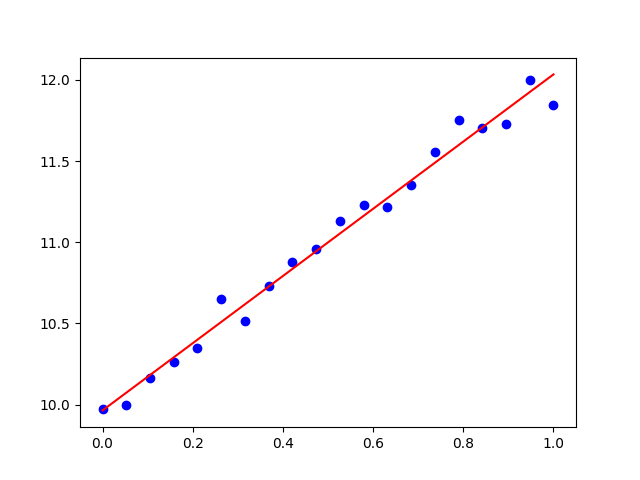
\includegraphics[width=0.75\textwidth]{fit_with_custom_callable.png}
  
  \medskip
  
  \begin{itemize}
    \item The fit works as usual
   \end{itemize}  
\end{frame}



\begin{frame}
  \frametitle{Summary}
  \begin{itemize}
    \item Special methods can beused to greatly enhance the readibility of the code
    \bigskip
    \item There are tens of special methods in python, covering logical operations,
          mathematical operations, array-style access, iterations, formatting and
          many other things\dots
    \bigskip
    \item Implementing the required interface in your classes you will be able
          to reuse a lot of code written for the standard containers thanks to
          duck typing, which is the pythonic way to polymorphism
   \end{itemize}  
\end{frame}






\end{document}
